%Here you can see how to include an image in your document.
%
%\begin{sidewaysfigure}
%\centering
%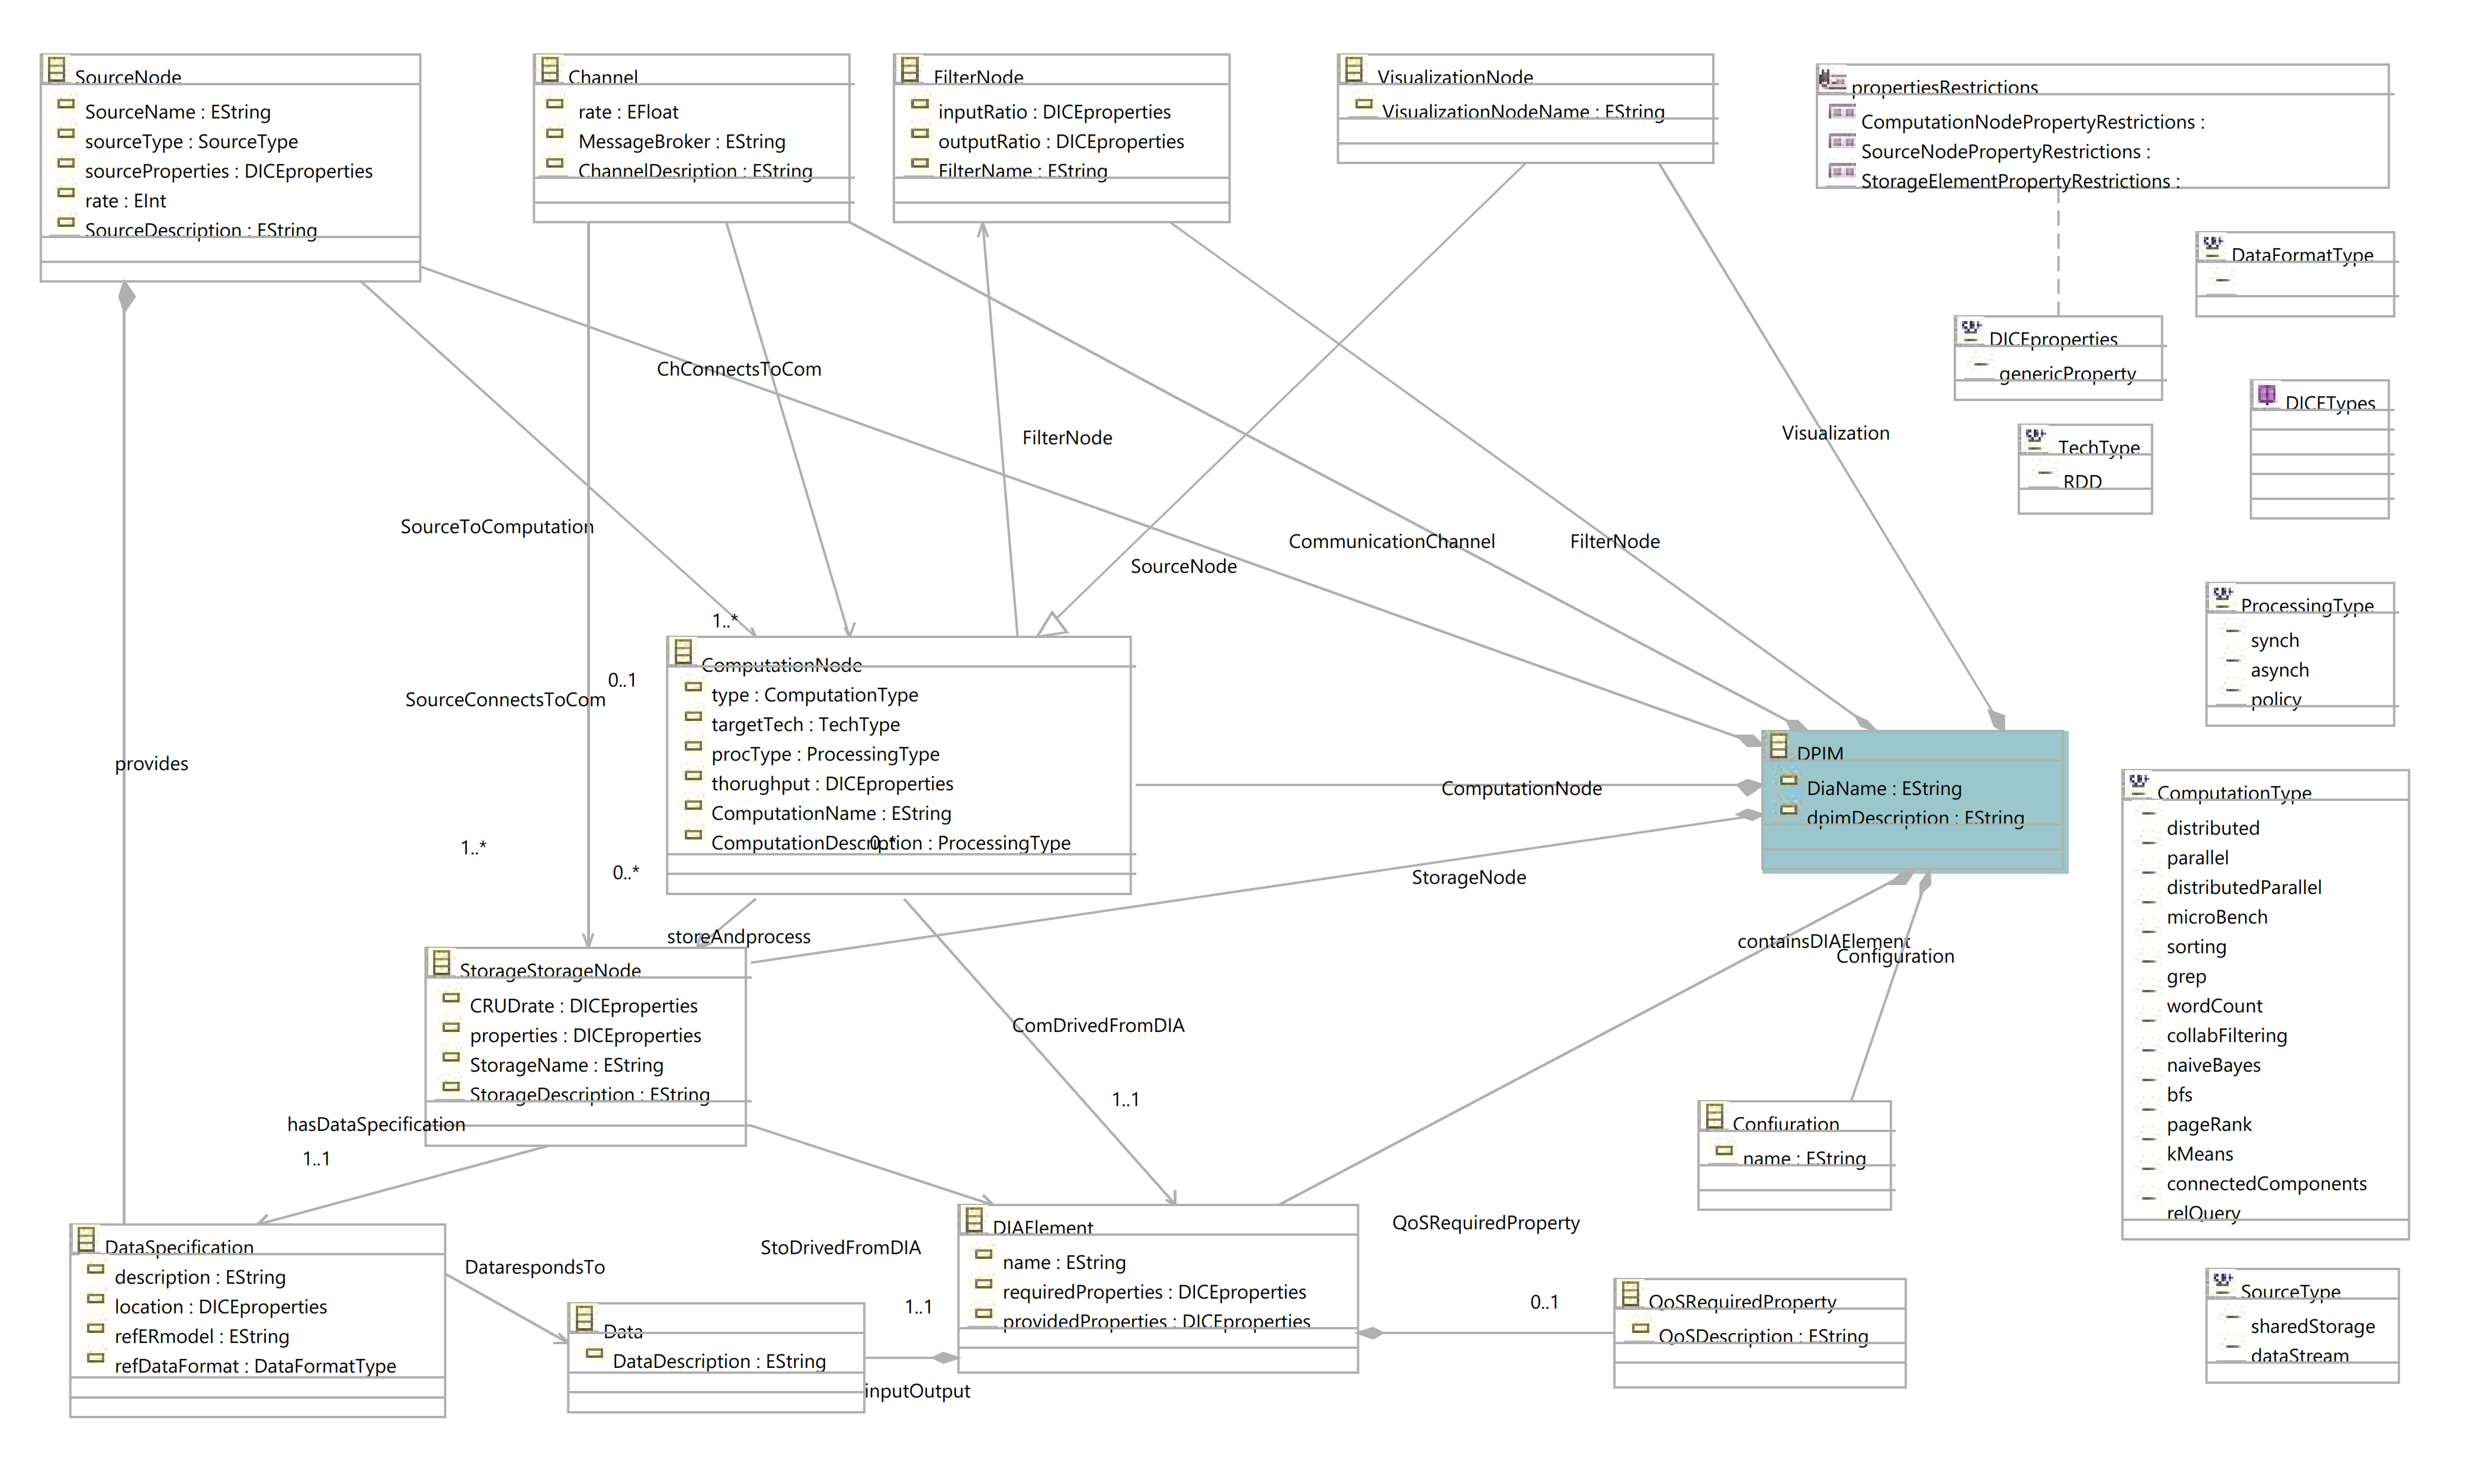
\includegraphics[width=\textwidth]{Images/11.png}
%\caption{\label{fig:metamodel}DICE DPIM metamodel.}
%\end{sidewaysfigure}

%\begin{figure}
%\centering
%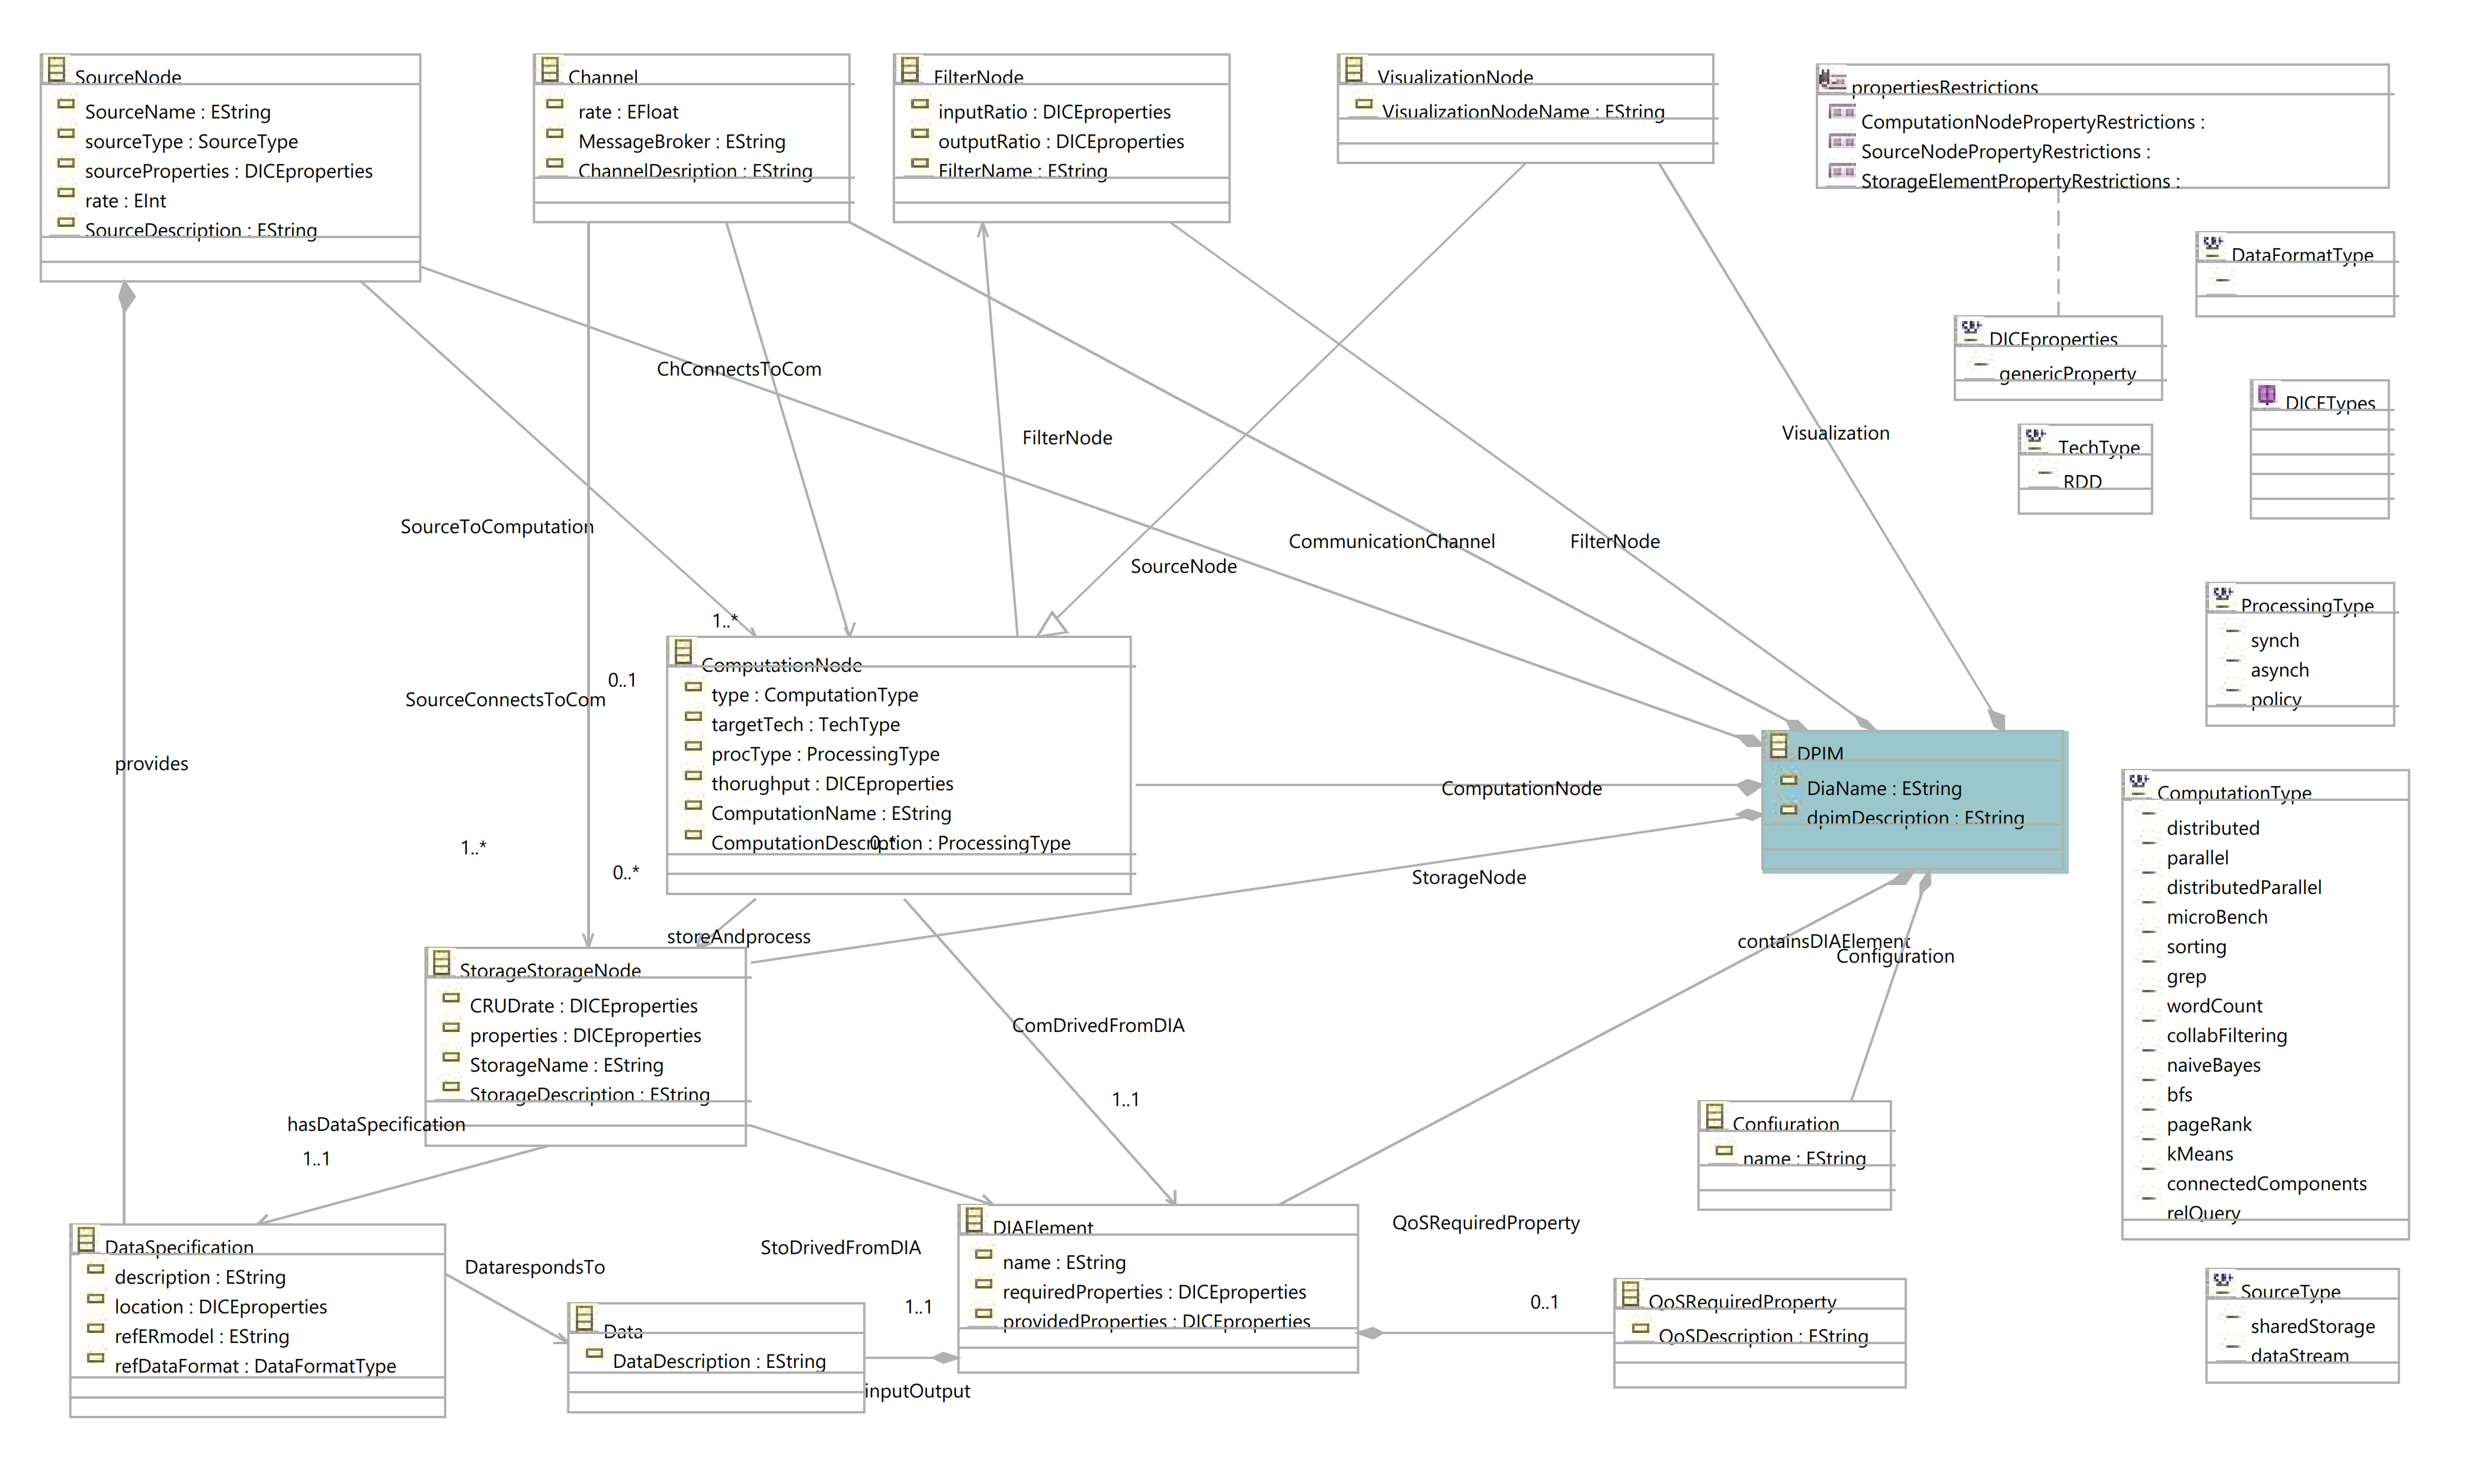
\includegraphics[width=\textwidth]{Images/11.png}
%\caption{\label{fig:metamodel2}DICE DPIM metamodel in portrait form.}
%\end{figure}

%Here is the command to refer to another element (section, figure, table, ...) in the document: \emph{As %discussed in Section~\ref{sect:overview} and as shown in Figure~\ref{fig:metamodel}, ...}. Here is how to %introduce a bibliographic citation~\cite{DAM}. Bibliographic references should be included in a \texttt{.bib} file. 

%Table generation is a bit complicated in Latex. You will soon become proficient, but to start you can %rely on tools or external services. See for instance this \href{https://www.tablesgenerator.com}{https://%www.tablesgenerator.com}. 

% -----------------------------------------------------
\subsection{Product perspective}

\subsubsection{Scenarios} 

\begin{enumerate}[label=\textbf{[\arabic*]}, left = 0 pt, align = left]
% ----
\item \textbf{A Student Registers on the Platform}:   
\\A student that is looking for an internship visits the S\&C platform for the first time. He or she decides to register to access potential internship opportunities.
They enter the Homepage and clicks on \textit{"Sign Up"}. At this point, a form appears where the student must insert his email, creates a password, and fills in their personal and academic details. After submitting the form, they quickly receive an email confirmation and follow the link to activate their account. 
Excited to start his search, the user logs in and begins creating his profile to make himself more visible to companies.

% ----
\item \textbf{Company Registration}:                                  
\\A company that is looking for interns visits the S\&C platform for the first time. It decides to register so it can access potential internship candidates. 
It enters the Homepage and clicks on \textit{"Sign In"}. At this point a form appears where the enterprise must insert the company name, the company email and creates a password. After submitting the form, it quickly receives an email confirmation and follows the link to activate its account. 
Excited to find the right candidates, the company logs in and begins creating its profile to make its internships more visible to prospective interns.

% ----
\item \textbf{Student Profile Creation}:  
\\Once a student logs into the platform, they can click on the \textit{"Edit profile"} button, which will redirect to a dedicated webpage displaying all the information required for the registration, along with a form that they can fill out. The student can add \textit{Basic Information}, \textit{Academic Information}, and \textit{Skills and Expertise} (like technical skills, soft skills, and certifications).
They can also include \textit{Experience and Achievements}, \textit{Internship Preferences}, \textit{CV}, \textit{Portfolio/Projects}, and \textit{Languages Spoken}

%####################
% ----
\item \textbf{Company Profile Creation}: 
\\Once a company logs into the platform, it can access to its profile by clicking on the icon in the
top-right corner of the screen. This directs the company to its profile page, where it can select the \textit{"Edit Profile"} button to add or modify information. Here, the company can fill details to personalize its profile, such as \textit{Basic Information} and \textit{Internship Program Details}.
The company can also include \textit{Testimonials} from former interns or current employees, enhancing its profile by showcasing the company culture and employee experiences.

% ----
\item \textbf{Internship Posting by Company}:                          
\\After setting up its profile, the company can post available internships by navigating to the internship creation section. Here, it can specify \textit{Internship Role Description} details, including the role title, responsibilities, required skills and qualifications, and the application process.
The company can also provide \textit{Application Details}, which feature an \textit{"Apply Now"} button for candidates and any required documents. It may also list \textit{Perks and Benefits} associated with the internship, such as compensation, additional benefits, and other perks to make the position more attractive to prospective interns.
%########################

% ----
\item \textbf{A Student Proactively Searches for an Internship}:                    
\\Once a student logs into the platform, he or she can easily find the \textit{"Available job search"} button. By clicking it the student will be redirected to another page of the website where they can type into the search bar specific keywords or they can apply specific filters on the search. Once the \textit{"Search"} button has been clicked, the user will see a list of suitable internship positions with synthetic details about the company which is offering it. If no internship matches the search criteria then the page will show a message stating the fact that no matches were found.

% ----
\item \textbf{A Student Actively Searches for a Match}:                   
\\Once a student registered to the platform fills or updates his/her profile with his information, he or she can click the button \textit{"Match me"} on his profile. Then, the platform runs analytics to match it with as many companies as possible. The profile of the student features a section with \textit{"Matching Internships"} where there is a list of all the suitable internships for him/her.

% ----
\item \textbf{A Company ???}   
\\Once a student registered to the platform fills or updates his/her profile with his information, he or she can then click the button \textit{Match Me} on his profilee platform runs analytics to match it with as many companies as possible. The profile of the student features a section with \textit{Matching Internships} where there is a list of all the suitable internships for him/her, relative to up to date information.

% ----
\item \textbf{Student Application to Internship}                      
\\Once a student finds an internship that might interest them, they can click on the preview of the placement, which will redirect to the company's private webpage. By pressing the \textit{"Apply Now"} button, a form will appear where the student must enter all the required information specified by the company. Once all the fields are completed, they can submit their application by clicking the \textit{"Submit"} button.

% ----
\item \textbf{Company Review of Student Applications}                
\\Once a company has posted one or more internship proposals, it will be able to see the applications submitted for each proposal by clicking on \textit{"Sent applications"}, which will redirect to a dedicated webpage displaying all the applications for a particular internship. For each application, brief information is shown on the screen, and the company can access the complete details by clicking the \textit{"More details"} button. If the company is interested to the student, it can click on \textit{"Start Selection Process"} to begin evaluating the candidate.

% ----
\item \textbf{Student Interview Scheduling}                          
\\


\item \textbf{Interview Conducted by Company}                        
\\


\item \textbf{Company Selection of Candidate}                        
\\


\item \textbf{Internship Offer Extended to Student}                  
\\


\item \textbf{Internship Offer Acceptance by Student}                
\\


\item \textbf{Feedback Submission by Student Post-Internship}        
\\


\item \textbf{Feedback Submission by Company Post-Internship}        
\\


\item \textbf{Statistical Analysis of Internship Matches}            
\\


\item \textbf{Internal Status Update by Student}                     
\\


\item \textbf{Internship Status Update by Company}                   
\\


\item \textbf{Notification of New Internship Opportunities}          
\\

\end{enumerate}

\subsubsection{Domain Class Diagram}

\subsubsection{State Diagrams}

% -----------------------------------------------------
\subsection{Product Functions}

% -----------------------------------------------------
\subsection{User Characteristics}

% one subsubsection for each type of user
\subsubsection{-}

% ------------------------------------------------------
\subsection{Assumptions, Dependencies and Constraints}

\subsubsection{Regulatory Policies}

\subsubsection{Domain Assumptions}
